\documentclass{article}
\usepackage{xeCJK}
\usepackage{amsmath, amsthm, amssymb}
\usepackage{hyperref}
\usepackage{listings}
\usepackage{xcolor}
\usepackage{bm}
\usepackage{graphicx}
\definecolor{dkgreen}{rgb}{0,0.6,0}
\definecolor{gray}{rgb}{0.5,0.5,0.5}
\definecolor{mauve}{rgb}{0.58,0,0.82}

\lstset{
  frame=tb,
  aboveskip=3mm,
  belowskip=3mm,
  showstringspaces=false,
  columns=flexible,
  framerule=1pt,
  rulecolor=\color{gray!35},
  backgroundcolor=\color{gray!5},
  basicstyle={\small\ttfamily},
  numbers=left,
  numberstyle=\tiny\color{gray},
  keywordstyle=\color{blue},
  commentstyle=\color{dkgreen},
  stringstyle=\color{mauve},
  breaklines=true,
  breakatwhitespace=true,
  tabsize=3,
  title=\lstname
}


%\DeclareMathOperator*{\Pr}{Pr}
\begin{document}
\title{第二次作业}
\author{赵丰,2017310711}
\maketitle
\section{理论题目}
\textbf{P1(a)}
因为$N$个点线性可分,所以存在由$\bm{a},b$确定的超平面
$\mathcal{H}=\{\bm{x}\in \mathcal{R}^d|\bm{a}^T\bm{x}+b=0\}$,
使得$\mathcal{H}$分离两类样本点,且分离的$margin$为$\rho$,即满足:
\begin{equation}
\begin{cases}
\bm{a}^T \bm{x}_i + b \leq -\frac{\rho}{2} & \text{if } y_i=-1\\
\bm{a}^T \bm{x}_i + b \geq \frac{\rho}{2} & \text{if } y_i=1 
\end{cases}
\end{equation}
取$t=\displaystyle\max_{1\leq i\leq N} ||\bm{x}_i||$,并令$\hat{\bm{w}}=(\frac{2t\bm{a}}{\rho},\frac{2tb}{\rho})$
,则可以直接验证
\begin{equation}
y_i \hat{\bm{w}}^T \bm{z}_i \geq 1, \forall i\in \{1,\dots,N\}
\end{equation}
\textbf{P1(b)}
\begin{align}
||\bm{w}_t-\hat{\bm{w}}||^2-||\bm{w}_{t+1}-\hat{\bm{w}}||^2=& 2(\bm{w}_{t+1}-\bm{w}_{t})\cdot \hat{\bm{w}}+(||\bm{w}_{t}||^2-||\bm{w}_{t+1}||^2)\\
=& 2y_i(\bm{z}_i)\cdot \hat{\bm{w}} +(||\bm{w}_{t}||^2-||\bm{w}_{t}+y_i\bm{z}_i||^2)\\
\geq & 2 - 2y_i\bm{w}_t\cdot \bm{z}_i +y_i^2||\bm{z}||^2\\
\geq & 1,y_i\bm{w}_t\cdot \bm{z}_i<0,||\bm{z}||=1 
\end{align}
因此$0\leq ||\bm{w}_t-\hat{\bm{w}}|| \leq ||\bm{w}_0-\hat{\bm{w}}||-t$,所以迭代次数$t\leq ||\bm{w}_0-\hat{\bm{w}}||$,
向上取整即得要证的结论。

\textbf{2.1(a)}
\begin{equation}
F(\bm{W})=\frac{1}{N}\bm{W}^T\bm{X}\bm{X}^T\bm{W}-\bm{W}^T\bm{X}\bm{Y}-\bm{Y}\bm{X}^T\bm{W}+\bm{Y}^T\bm{Y}
\end{equation}
令$\frac{\partial F(\bm{W})}{\partial \bm{W}}=\bm{0}$,解出
$\bm{W}=(\bm{X}\bm{X}^T)^{-1}\bm{X}\bm{Y}$即为最优解。

\textbf{2.1(b)}
设$\bm{v}\in \mathcal{R}^N$,则$(\bm{X}\bm{X}^T)^{-1}\bm{X}\bm{v}\in \mathcal{R}^{d+1}$,因此
$\bm{X}^T(\bm{X}\bm{X}^T)^{-1}\bm{X}\bm{v}$是$\bm{X}^T$各列向量的线性组合,落在由$\bm{X}^T$列向量张成的线性空间中。

为证$\bm{X}^T(\bm{X}\bm{X}^T)^{-1}\bm{X}\bm{Y} - \bm{Y}$与$\bm{X}^T$列向量张成的线性空间正交,只需证
$\bm{X}^T(\bm{X}\bm{X}^T)^{-1}\bm{X}\bm{Y} - \bm{Y}$与$\bm{X}^T$各列向量垂直。即证
$(\bm{X}^T)^T \left(\bm{X}^T(\bm{X}\bm{X}^T)^{-1}\bm{X}\bm{Y} - \bm{Y}\right)=0$,化简即得。

\textbf{2.2}
设
\begin{equation}
h_w(\bm{x})=\frac{1}{1+exp(-\bm{w}^T\bm{x})}
\end{equation}
对于Logistic Model,对数似然函数为
\begin{equation}
\log L(\bm{w}|\bm{x})=\sum_{i=1}^m y_i \log h_w(\bm{x}_i) + (1-y_i) \log (1-h_w(\bm{x}_i))
\end{equation}
对$\bm{w}$求导得
\begin{equation}
\sum_{i=1}^m(h_w(\bm{x}_i)-y_i)\bm{x}_i=0
\end{equation}
上面方程关于$h_w(\bm{x}_i)$的最小二乘解为$h_w(\bm{x}_i)=y_i$,我们假设$y_i$取$\pm 1$,因为原数据集线性可分,所以存在$\bm{w'}$,使得
$\bm{w'}^T\bm{x}_i>0$对$y_i=1$成立,此时$\frac{1}{1+exp(-\bm{w'}^T\bm{x}_i)}>\frac{1}{2}$,增大$\bm{w'}$的模长使得
$\frac{1}{1+exp(-\bm{w'}^T\bm{x}_i)}$更接近1。对于$y_i=-1$有类似的观察,因此MLE方法对Logistic Model给出的$\bm{w}$可以沿着$\bm{w'}$的方向将其模长取到任意大得到。

\textbf{2.3}
% 均方误差$E$为
% \begin{equation}
% E=\frac{1}{2}\sum_{i=1}^M (\bm{w}^T \bm{x}_i+w_0-y_i)^2
% \end{equation}
% 取$E$对$w_0$的偏导数为0,得
% \begin{equation}
% \sum_{i=1}^M (\bm{w}^T \bm{x}_i+w_0-y_i)=0
% \end{equation}
% 由于有$M_1$个样本点取值为$\frac{M}{M_1}$,$M_2$个样本点取值为$-\frac{M}{M_2}$,所以
% $\displaystyle\sum_{i=1}^M y_i=0,因此由上式求出$w_0=-\bm{w}^T\bm{m}$。
已知
\begin{equation}
\bm{m}_1=\frac{1}{M_1}\sum_{n\in C_1} \bm{x}_n,\bm{m}_2=\frac{1}{M_2}\sum_{n\in C_2} \bm{x}_n
\end{equation}
\begin{align*}
&\sum_{i=1}^M (\bm{w}^T\bm{x}_i+w_0-y_i)\bm{x}_i=0\\
\iff & \sum_{n \in C_1}^M (\bm{w}^T\bm{x}_i+w_0-y_i)\bm{x}_i+\sum_{n \in C_2}^M (\bm{w}^T\bm{x}_i+w_0-y_i)\bm{x}_i=0\\
\iff & \sum_{n \in C_1}^M (\bm{w}^T\bm{x}_i-\bm{w}^T\bm{m}-\frac{M}{M_1})\bm{x}_i+\sum_{n \in C_2}^M (\bm{w}^T\bm{x}_i-\bm{w}^T\bm{m}+\frac{M}{M_2})\bm{x}_i=0\\
\iff & \sum_{n \in C_1}^M (\bm{w}^T\bm{x}_i)\bm{x}_i+\sum_{n \in C_2}^M (\bm{w}^T\bm{x}_i)\bm{x}_i-(\bm{w}^T\bm{m}+\frac{M}{M_1})M_1\bm{m}_1+(-\bm{w}^T\bm{m}+\frac{M}{M_2})M_2\bm{m}_2=0\\
\iff & \underbrace{\sum_{n \in C_1}^M (\bm{x}_i\bm{x}_i^T)\bm{w}}_{I_1}+\underbrace{\sum_{n \in C_2}^M (\bm{x}_i\bm{x}_i^T)\bm{w}}_{I_2}+\underbrace{(-M_1\bm{w}^T\bm{m}-M)\bm{m}_1+(-M_2\bm{w}^T\bm{m}+M)\bm{m}_2}_{I_3}=0\\
\end{align*}
\begin{align*}
I_1 =&  \sum_{n \in C_1}^M (\bm{x}_i\bm{x}_i^T)\bm{w} \\
=& \sum_{n \in C_1}^M \left( ((\bm{x}_i-\bm{m}_1)(\bm{x}_i-\bm{m}_1)^T)\bm{w}+(\bm{m}_1\bm{x}_i^T)\bm{w}+(\bm{x}_i\bm{m}_1^T)\bm{w}-(\bm{m}_1\bm{m}_1^T)\bm{w}\right)\\
=& \sum_{n \in C_1}^M \left( ((\bm{x}_i-\bm{m}_1)(\bm{x}_i-\bm{m}_1)^T)\bm{w}\right)+M_1(\bm{m}_1\bm{m}_1^T)\bm{w}\\
\end{align*}
同理
\begin{equation}
I_2=\sum_{n \in C_2}^M \left( ((\bm{x}_i-\bm{m}_2)(\bm{x}_i-\bm{m}_2)^T)\bm{w}\right)+M_2(\bm{m}_2\bm{m}_2^T)\bm{w}
\end{equation}
因此
\begin{equation}
I_1+I_2=S_W\bm{w}+M_1(\bm{m}_1\bm{m}_1^T)\bm{w}+M_2(\bm{m}_2\bm{m}_2^T)\bm{w}
\end{equation}
\begin{align*}
I_3 = & (-M_1\bm{w}^T\bm{m}-M)\bm{m}_1+(-M_2\bm{w}^T\bm{m}+M)\bm{m}_2\\
= & (-M_1\bm{w}^T\frac{M_1\bm{m}_1+M_2\bm{m}_2}{M}-M)\bm{m}_1+(-M_2\bm{w}^T\frac{M_1\bm{m}_1+M_2\bm{m}_2}{M}+M)\bm{m}_2\\
= & (-M_1\frac{M_1\bm{m}_1\bm{m}_1^T+M_2\bm{m}_2\bm{m}_1^T}{M})\bm{w}+(-M_2\frac{M_1\bm{m}_1\bm{m}_2^T+M_2\bm{m}_2\bm{m}_2^T}{M})\bm{w}-M(\bm{m}_1-\bm{m}_2)\\
\end{align*}
\begin{align*}
&I_1+I_2+I_3=0\\
\iff & S_W\bm{w}+M_1(\bm{m}_1\bm{m}_1^T)\bm{w}+M_2(\bm{m}_2\bm{m}_2^T)\bm{w}+(-M_1\frac{M_1\bm{m}_1\bm{m}_1^T+M_2\bm{m}_2\bm{m}_1^T}{M})\bm{w}\\
+&(-M_2\frac{M_1\bm{m}_1\bm{m}_2^T+M_2\bm{m}_2\bm{m}_2^T}{M})\bm{w}-M(\bm{m}_1-\bm{m}_2)=0\\
\iff & S_W\bm{w}+\frac{1}{M}(M_1(M_1+M_2)(\bm{m}_1\bm{m}_1^T)+M_2(M_1+M_2)(\bm{m}_2\bm{m}_2^T)-M_1^2\bm{m}_1\bm{m}_1^T-M_1M_2\bm{m}_2\bm{m}_1^T\\
-&M_1M_2\bm{m}_1\bm{m}_2^T-M_2^2\bm{m}_2\bm{m}_2^T)\bm{w}-M(\bm{m}_1-\bm{m}_2)=0\\
\iff & (S_W+\frac{M_1M_2}{M}S_B)\bm{w}-M(\bm{m}_1-\bm{m}_2)=0
\end{align*}

\textbf{3(a)}
设
\begin{align}\notag
L(\bm{u},\bm{v},\bm{w},\bm{\xi},\bm{\alpha},b)=&
\frac{1}{2}||\bm{\alpha}||_2^2+C ||\bm{\xi}||_1-\sum_{i=1}^m u_i
\left(y_i(\sum_{j=1}^m \alpha_j y_j \bm{x}_i^T\bm{x}_j +b)-1+\xi_i\right) \\
-&\sum_{i=1}^m v_i \xi_i -\sum_{i=1}^m w_i\alpha_i
\end{align}
原优化问题的Lagrange对偶为:
\begin{align}\notag
\max & \inf_{\bm{\xi},\bm{\alpha},b}{L(\bm{u},\bm{v},\bm{w},\bm{\xi},\bm{\alpha},b)}\\
\text{s.t.}\,\, & \bm{u},\bm{v},\bm{w}\geq 0\label{eq:dual}
\end{align}
$L$分别对各个变量求偏导数,得
\begin{align}
\alpha_j-\sum_{i=1}^m (u_i y_iy_j \bm{x}_i^T\bm{x}_j)-w_j=&0,j=1,2,\dots,m\label{eq:alpha}\\
C-u_i-v_i =& 0 \label{eq:uConstraint}\\
\sum_{i=1}^m u_i y_i =&0
\end{align}
将\eqref{eq:alpha}式求出的$\bm{\alpha}$代入\eqref{eq:dual}式,得到
$\inf L$为
\begin{equation}
\mathcal{L}=-\frac{1}{2}\sum_{i=1}^m w_i^2 -\frac{1}{2}\sum_{i=1}^m\left(\sum_{j=1}^m u_j y_iy_j \bm{x}_i^T\bm{x}_j\right)^2
-\sum_{i,j=1}^m (y_i y_j \bm{x}_i^T\bm{x}_j) u_i w_j+\sum_{i=1}^m u_i
\end{equation}
由\eqref{eq:uConstraint}式,关于$\bm{v}$的约束可以转化为$u_i\leq C$,因此\eqref{eq:dual}式化简为:
\begin{align}\notag
\max_{\bm{u},\bm{w}} & -\frac{1}{2} \sum_{i=1}^m w_i^2 -\frac{1}{2}\sum_{i=1}^m\left(\sum_{j=1}^m u_j y_iy_j \bm{x}_i^T\bm{x}_j\right)^2
-\sum_{i,j=1}^m (y_i y_j \bm{x}_i^T\bm{x}_j) u_i w_j+\sum_{i=1}^m u_i\\
\text{s.t.}\,\, & w_j\geq 0, 0\leq u_j \leq C, \bm{u}^T\bm{y}=0
\end{align}
注意到对偶问题是关于$\bm{u},\bm{w}$的带有区间不等式约束的二次规划问题。
$u_iu_k$的系数为$(y_j \bm{x}_j)^T(\sum \bm{x}_i\bm{x}_i^T) (y_k \bm{x}_k)$,具有内积的表达形式,因此目标函数是约束变量的凸函数,
可采用凸优化的方法求解对偶问题。

\textbf{3(b)}
考虑关于$\bm{\alpha}$的1范数,
\begin{align}\notag
L(\bm{u},\bm{v},\bm{w},\bm{\xi},\bm{\alpha},b)=&
||\bm{\alpha}||_1+C ||\bm{\xi}||_1-\sum_{i=1}^m u_i
\left(y_i(\sum_{j=1}^m \alpha_j y_j \bm{x}_i^T\bm{x}_j +b)-1+\xi_i\right) \\
-&\sum_{i=1}^m v_i \xi_i -\sum_{i=1}^m w_i\alpha_i\label{eq:p1}
\end{align}
此时\eqref{eq:alpha}式变为
\begin{equation}
1-\sum_{i=1}^m (u_i y_iy_j \bm{x}_i^T\bm{x}_j)-w_j=0,j=1,2,\dots,m
\end{equation}
代入\eqref{eq:p1}式中,得对偶问题为
\begin{align}\notag
\max_{\bm{u}} & \sum_{i=1}^m u_i\\
\text{s.t.}\,\, & 0\leq u_j \leq C, \\
&\bm{u}^T\bm{y}=0,\\
&1-\sum_{i=1}^m (u_i y_iy_j \bm{x}_i^T\bm{x}_j)\geq 0,j=1,2,\dots,m
\end{align}

\section{Program Practice}
使用Logistic 方法和SVM 方法分别对给定的数据进行2分类,
\subsection{Logistic Regression}
Doing:
针对给定的数据,首先采用线性归一化的方法将每一维数据压缩到$[0,1]$区间上。

\textbf{a}:
采用 Gradient Ascent Method 而不是求解非线性方程的方法更新模型参数:
迭代公式为:
\begin{equation}
\bm{w}\leftarrow \bm{w}+\alpha(y_i-h_w(\bm{x}_i)\bm{x}_i
\end{equation}
具体更新时可用训练集多次迭代直到误差不再下降为止。

\textbf{b}:
在似然函数中加入先验(正则因子)$\frac{\lambda}{2} ||\bm{w}||^2$,其中$\lambda$
为正则化因子。在给定$\lambda$的情形下,对似然函数关于$\bm{w}$求梯度得非线性方程:
\begin{equation}\label{eq:EGradient}
\nabla_{\bm{w}}\mathcal{L}(\bm{w})=\lambda \bm{w}+\sum_{i=1}^{m}(y_i-h_w(\bm{x}_i))\bm{x}_i=0
\end{equation}
其中有$m$个训练数据。根据下面的IRLS方法的启示,可以用Newton 迭代法求解上面的
非线性方程,只不过此时以\eqref{eq:EGradient}为梯度,Hessian 矩阵为:
\begin{equation}
H=-\bm{X}\bm{R}\bm{X}^T+\lambda \bm{I}
\end{equation}
其中$\bm{X}=[\bm{x}_1,\dots,\bm{x}_m]$是$n\times m$的矩阵, 
$\bm{R}$是对角阵,如设$u_i=h_w(\bm{x}_i)(1-h_w(\bm{x}_i))$,则对角元为$R_{ii}=u_i(1-u_i)$
$H$的阶数与$\bm{w}$的维数相同,通过加上一个$\lambda \bm{I}$的单位阵可以改善$H$的正定性质。
于是我们的迭代步为:
\begin{equation}
\bm{w}_{t+1}=\bm{w}_t+(\bm{X}\bm{R}\bm{X}^T+\lambda \bm{I})^{-1}(\bm{X}(\bm{y}-\bm{u})+\lambda \bm{w}_t)
\end{equation}
$\bm{u},\bm{y}$是$m$维的向量

我们首先把把数据集分成5份,选不同的$\lambda$代入计算,每次计算中,分5轮,每一轮中以4份训练1分验证,
5次结果取平均得到错误率。

Report:

\textbf{a}:
由于全部数据均带有标记,可以将其按照4:1的关系分为训练数据和测试数据,
其中训练数据用于训练模型参数,然后在测试数据上进行预测。

\textbf{b}:
对于正则化的Logistic 回归,我们通过调整正则化参数,得到其在测试集上最小的预测误差为$0.31$。并且在正则化参数接近0时取得,
结果与IRLS方法的预测误差近似。
\begin{figure}[!ht]
\centering
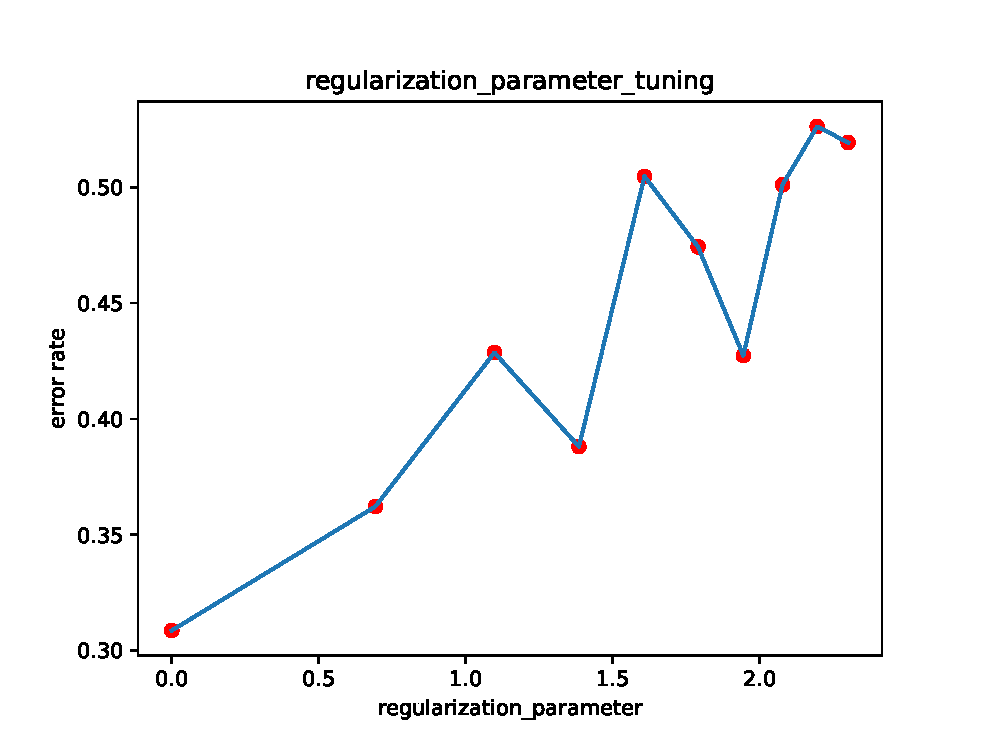
\includegraphics[width=7cm]{logistic_regression_regularization_parameter_tuning.eps}
\end{figure}

\textbf{c}:
以IRLS方法为例,我们按$d\%$抽取训练集,其余数据作为测试集,以训练集的百分比为横轴,以误差为纵轴,分别画出
训练出的模型在训练集和测试集上的误差曲线如下所示:

\begin{figure}[!ht]
\centering
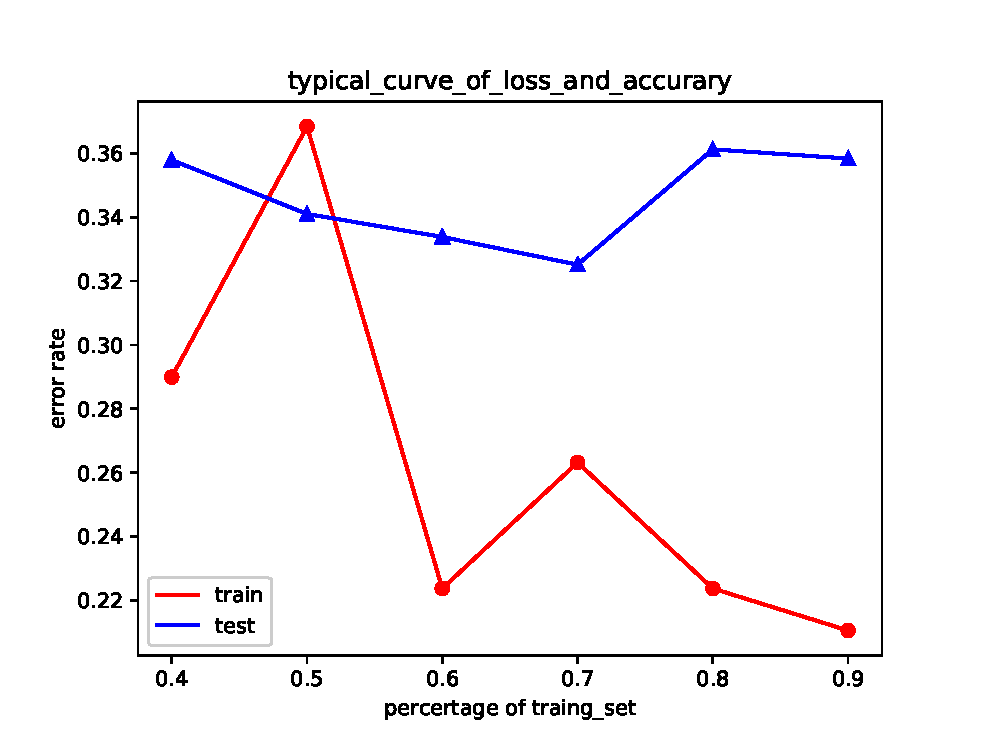
\includegraphics[width=7cm]{typical_curve_of_loss_and_accurary.eps}
\end{figure}

从上图可以看出,当训练集用的比重过大时,尽管在训练集上的误差下降到了30\%以下,但在测试集上的误差却有明显上升,即
出现了明显的过拟合的问题。

对于标准的随机梯度方法,我们得到测试集上的准确率为$0.32\pm 0.04$,对于IRLS方法,准确率为$0.31\pm 0.04$,
IRLS方法略优于随机梯度法,但计算开销方面却较大。

\textbf{d}:
我们以训练集的经验误差不再下降作为模型参数迭代是否终止的标准,根据算法实现的结果来看,随机梯度方法需要在全部的训练
数据上跑1到2次经验误差不再下降,而IRLS方法需跑2到3次。

\subsection{SVM}
Doing:

\textbf{b}:
我们采用 Linear Kernel, Gaussian Kernel%
%radial basis function
分别作为核函数,它们分别有0,1个额外参数必须提前确定才能求解
凸优化问题确定支持向量,另外还有正则化因子需要确定。因此我们针对两种核函数模型,采用Grid Search 与控制变量相结合的方法
寻找使判别误差最小的Hyper-parameters 的取值。


同样的,我们对数据进行适当的归一化后进行训练和预测。

Report:

\textbf{a}:
\begin{figure}[!ht]
\centering
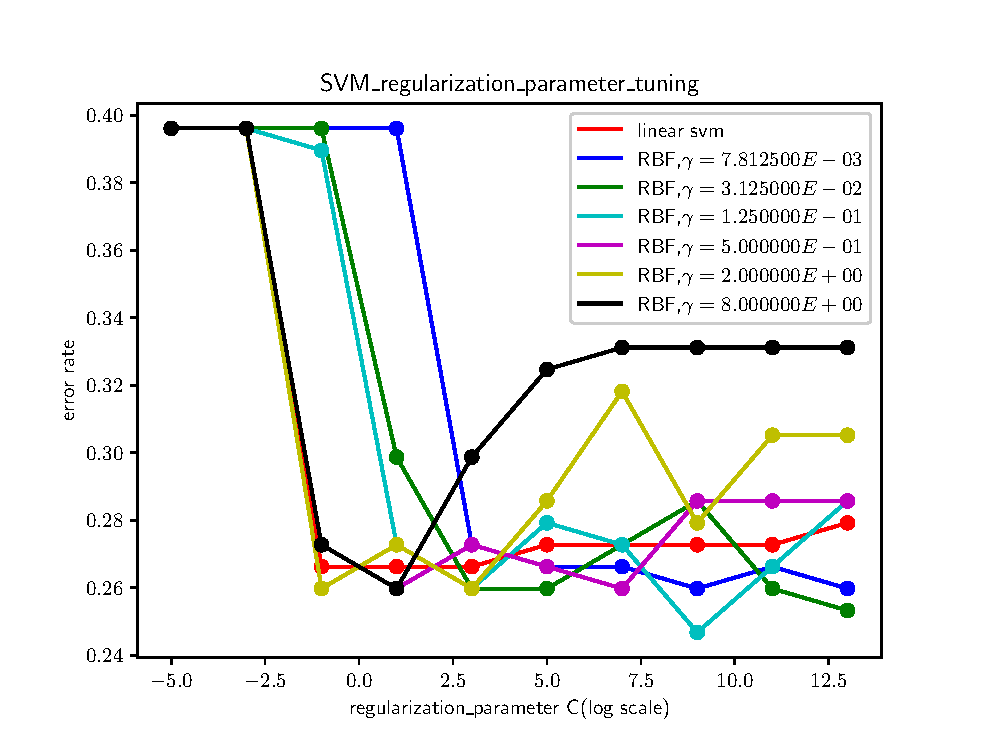
\includegraphics[width=9cm]{SVM_regularization_parameter_tuning.eps}
\end{figure}

由上图可知,取RBF核函数,$C \approx a,\gamma \approx b$时可取得最小的预测误差值,约为$c$,该模型的预测误差比
其他线性方法均要小。

上机作业使用的Python代码:

\lstinputlisting[language=Python]{diabetes.py}

\begin{equation}
\end{equation}

\end{document}
